\chapter{Linear Transformations}

In this chapter we focus on linear transformations in metric spaces. Recall that the term \emph{linear transformation} means a linear function that takes in one type of object and returns the same type of object. The linearity means that a linear combination of inputs returns a linear combination of outputs. In this course, we reserve the word \textbf{matrix}\index{linear transformation} to mean a linear transformation. We observed that a matrix $M\aij{i}{j}\ket{e_i}\!\bra{e_j}$ can equivalently take in a vector or a row vector and output an object of the same class. 


\section{The hierarchy of transformations}
\label{sec:hierarchy:of:transformations}

There is something odd that I do when I think about mathematical objects. I impose upon these objects some subjective feeling of niceness or not-niceness. Nice matrices are easy to use. The nicest matrices are easy to undo. Matrices that are not nice may be complicated---perhaps they are a complicated manifestation of something which is supposed to be simple. Another not-nice feature is if a matrix is not invertible: once you apply it, the object on which you have applied it has lost information. The worst matrices do not fall into these categories. There is one step below `worst': matrices that are not even matrices by our definition, for example linear maps that do not return vectors in the same vector space as the input.\sidenote{There are even worse (worser?) ``matrices'' like the $N\times (N+1)$ objects you write down to do weird shit like ``reduced row echelon form'' in a traditional linear algebra class. That's just solving a system of linear equations---that's just algebra, it is not even \emph{linear algebra}.}

The following hierarchy of matrices is not official. It is not found in any textbook of mathematics or physics. In fact, I would vehemently deny that I even taught this to you.\sidenote{This reminds me of the advice my Ph.D advisor gave me when I asked what I should do if my first seminar talk does not go well. He told me, ``If it goes \emph{really} poorly, then lie about who your advisor is.''} However, it does help me categorize the types of matrices that \emph{do} show up in physics and how to think about them.\sidenote{You may compare this to what psychologist refer to as Maslow's hierarchy of needs.}

\begin{enumerate}
    \item The top-of-the line, S-rank, nicest matrices are \textbf{multiples of the identity}. These are just numbers: not only are they defined by a single proportionality constant, but they add and multiply as if they are just numbers. Unfortunately, these matrices are \emph{too} nice: all they do is rescale the vector or dual vector that they act on. That is a little boring, even for us.
    \item The A-class matrices are \textbf{diagonal} in the basis you are currently using. We also assume that each of the diagonal elements are non-zero.\sidenote{We say the matrix is \emph{non-degenerate}.} In this basis, the matrix acts by rescaling each component of a vector or row vector. Each component is stretched or shrunk independently: that means that the resulting vector could look rather different. Most of the time we specialize to the case where the diagonal elements are positive.
    \item At \emph{almost} the same level as the diagonal matrices are matrices that are \textbf{diagonalizable} and, when diagonalized, have no zero elements along the diagonal. The verb `to diagonalize' means that there is some \emph{isometry} (rotation) where we may change basis and the components of $A$ would be diagonal. Most of our active transformations in physics---the ones where we ``do something''---take this form. Because diagonal matrices are so nice, it then behooves us to take these matrices and rotate into the proper basis where they are diagonal.\sidenote{This is called the eigenbasis or basis of eigenvectors. The word `eigen' means `proper' in German. At least I think that's what it means. The diagonal components of the matrix in the eigenbasis are called eigenvalues.}
    \item Now I pause to (re-)define a different class of matrices, \textbf{isometries}. Isometries are transformations that preserve the form of the metric. In some sense, they should not even be on this list since they are most naturally understood as \emph{passive} transformations---see Section~\ref{sec:active:passive}. They are a special class because we use these isometries to go into a basis where matrices are diagonal.\sidenote{In my brain diagonalizing matrices is ``doing [the] eigenstuff.''} Even among isometries, there are two types depending on whether or not they preserve the orientation of your basis.\sidenote{This is a matter of whether or not you change the \emph{handedness} of your basis.}
    \item There are matrices that are not so `nice' but are often meaningful and useful. These are called \textbf{projections}. These are matrices that are not invertible because they remove information from the vectors that they act on. A good example is a diagonal matrix with at least one zero diagonal component. When that matrix acts on a vector, the information of that component is completely lost---there is no way to recover it based on the output vector. 
    \item The last useful type of matrix are those that are none of the above but are otherwise $N\times N$ matrices that take vectors from one vector space and return vectors in the same vector space. These may be random $N\times N$ matrices, for example. We neither expect them to be diagonalizable by a rotation nor are they obviously meaningful as projections. These matrices may still be diagonalized, but usually the transformation to do this is not a simple isometry. Further, the diagonal matrices may not necessarily be positive upon diagonalization.
    \item All other matrices---for example, $N\times M$ matries with $M\neq N$---are just completely off the table. 
\end{enumerate}

\begin{example}[Active versus passive] In a passive transformation, tensors do not transform. Instead, we are simply changing our basis---physically, we are changing our reference frame. For such a transformation, the components of a tensor change because the basis vectors change, even if the tensor itself remains the same. 

In an active transformation, the components of a tensor change but the basis remains the same. This corresponds to actually changing the tensor and not changing the observer.
\end{example}

\begin{exercise}
Draw a vector---any vector---in $\mathbbm{R}^2$. Act on this vector with the matrix, whose components we write with respect to the standard basis:
\begin{align}
    A = \begin{pmatrix}
        A\aij{1}{1} & A\aij{1}{2}\\
        A\aij{2}{1} & A\aij{2}{2}
    \end{pmatrix}
    =
    \begin{pmatrix}
        3 & 0\\
        0 & \frac{1}{2}
    \end{pmatrix} \ .
\end{align}
Draw the resulting vector. Do the same for the case with the same matrix except that $A\aij{1}{1} = -3$.
\end{exercise}


% Identity
% Diagonal
% Rotated from the diagonal: symmetric
% Projections
% All others
% not included: $N\times M$

\section{Non-invertible matrices}

The nicest matrices are invertible. In fact, most of the linear transformations you encounter in a physics curriculum are invertible simply because so many of the mathematical tasks in physics involve inverting the dynamics encoded in these matrices. It behooves us to say a few words about the types of matrices that are not so nice.

\subsection{A first look at projections}

Projections are the matrices that are non-invertible because they send some non-zero vector to zero. A simple example follows:
\begin{example}
Consider the matrix
\begin{align}
    M = 
    \begin{pmatrix}
        2 & 0 \\
        0 & 0
    \end{pmatrix} \ .
\end{align}
This matrix takes any vector oriented in the $\hat{e_2}$ direction to zero: $M\ket{e_2} = 0$. This means that the action of the matrix on a general vector $\ket{v} = v^i\ket{e_i}$ is
\begin{align}
    M \ket{v} = v^1 M\ket{e_1} = 2 v^1 \ket{e_1} \ .
\end{align}
It does not matter what $v^2$ is, the image of $M\ket{v}$ only depends on $v^1$. In this way, one has \emph{lost} information. If you know that
\begin{align}
    M\ket{v} = \ket{w}
    \label{eq:Mv:eq:w:projection:eg}
\end{align}
for some known vector $w^i\ket{e_i}$, then there is no way to figure out what $\ket{v}$ is uniquely because there is a degeneracy where any vector $\ket{v}$ satisfying \eqref{eq:Mv:eq:w:projection:eg}, any vector of the form $\ket{v} + \alpha\ket{e_2}$ will also satisfy \eqref{eq:Mv:eq:w:projection:eg}. 

In fact, you may notice that if $w^2 \neq 0$, then \eqref{eq:Mv:eq:w:projection:eg} has no solution.
\end{example}

\begin{exercise}
A slightly less trivial example is as follows:
\begin{align}
    M = 
    \begin{pmatrix}
        2 & 1 & 0 \\
        3 & 2 & 0 \\
        0 & 0 & 0
    \end{pmatrix} \ .
\end{align}
Verify that the image of any vector $\vec{v}$ does not contain any component in the $\ket{e_3}$ direction. Further verify that the image of any any vector $\vec{v}$ is independent of $v^3$.
\end{exercise}

Matrices of these types are projections. We discuss these more fully in Section~\ref{sec:projections}. When a matrix causes a non-zero vector to vanish, it is necessarily a projection.\footnote{A narrow definition of a projection is that most components of a vector are preserved while some are lost. An example of this is the matrix $\ket{e_2}\!\bra{e_2}$. However, for our purposes we use projection to mean any transformation that loses information.} A key theme is that one \emph{loses information} about the original vector $\vec{v}$ when acting on it with a projection. There is no way to unambiguously reconstruct $\ket{v}$ given its image $M\ket{v}$.



\subsection{Degenerate image}

You may think that the problem with the matrices in the example above is that there are too many zeros in the matrix. After all, these zeros throw away the dependence on components of the input vector. This is na\"ive: the numerical values of a matrix are basis-dependent. Here's another example:
% 
\begin{example}
The following matrix is degenerate:
\begin{align}
    M = 
    \begin{pmatrix}
        1 & 1 \\
        2 & 2
    \end{pmatrix} \ .
\end{align}
This matrix has no zero elements---at least not in this basis---but there's clearly something fishy about it. If you act on this matrix on any vector, you find that the result is proportional to $\ket{e_1} + 2 \ket{e_2}$. Go ahead, try it. 

One way to see this is that it takes both basis vectors $\ket{e_{1,2}}$ to
\begin{align}
    M\ket{e_{1,2}} = \ket{e_1} + 2 \ket{e_2} \ .
\end{align}
We see that $M$ is again non-invertible. Given some vector of the requisite form, $\ket{w} = \alpha \ket{e_1} + 2\alpha \ket{e_2}$, there is no unambiguous solution for $\ket{v}$ to the equation $M\ket{v} = \ket{w}$. We can show this simply by writing out two solutions that both gives the same $\ket{w}$:
\begin{align}
    \ket{v_I} &= \alpha \ket{e_1}
    &
    \ket{v_{II}} &= \alpha \ket{e_2} \ .
\end{align}
\end{example}
\begin{exercise}
In the previous example, show that the most general solution to $M\ket{v} = \ket{w}$ is
\begin{align}
    \ket{v} &= \beta\ket{e_1} + (\alpha-\beta)\ket{e_2} \ .
\end{align}
\end{exercise}
\begin{exercise}
In the previous example, argue that the matrix $M$ has many zeros in the basis
\begin{align}
    \ket{f_1}&= \frac{1}{\sqrt{2}}
    \left[\ket{e_1}+\ket{e_2}\right]
    &
    \ket{f_2}&= \frac{1}{\sqrt{2}}
    \left[\ket{e_1}-\ket{e_2}\right] \ .
\end{align}
\end{exercise}
The lesson from this section is that projections are not always so obvious by their zero components. 


\section{Action on basis vectors}

A linear transformation is defined by its action on basis vectors. Consider a matrix $M$ that is non-degenerate. A convenient way of stating this is that the action of $M$ onto each of the basis vectors $M\ket{e_i}$ produces a set of vectors that are \emph{linearly independent}.\sidenote{Unless $M$ is an isometry, the vectors $M\ket{e_i}$ are not orthonormal.} This is another way of saying that $M$ is invertible and so does not lose information. 
\begin{exercise}
In your own words, articulate why the linear independence of the $M\ket{e_i}$ image vectors implies that $M$ is invertible? \textsc{Hint}: one way to do this is to argue that a given vector $\ket{w}$ is the image of a unique vector $\ket{v}$ under $M$: $M\ket{v} = \ket{w}$.
\end{exercise}

This leads us to a useful point:
\begin{bigidea}
A linear transformation is defined---and completely described---by its action on the basis vectors of a vector space.
\end{bigidea}
We can see this by writing a vector as a linear combination of basis vectors, $\ket{v} = v^i\ket{e_i}$. Because $M$ is a linear transformation, knowing the action of $M$ on each $\ket{e_i}$ completely specifies the action of $M$ on the linear combination $\ket{v}$. 

What does it mean to know the action of $M$ on the basis vectors? $M$ maps each basis vector into some other vector. In general the image vector will not be normalized nor orthogonal to the images of other basis vectors. How does one describe the image vector? The obvious way is to give the components of $M\ket{e_i}$ with respect to the $\ket{e_i}$ basis. The component of $M\ket{e_i}$ in the $\ket{e^j}$ direction is simply
\begin{align}
    \la e^j \mid M \mid e_i \ra 
    = 
    \la e^j \mid M\aij{k}{\ell}\ket{e_k}\!\bra{e^\ell} \mid e_i \ra 
    = M\aij{j}{i} \ .
\end{align}
This is one of those \emph{aha} moments where you may first feel surprised that the components of $M\aij{j}{i}$ have popped out, but then you realize that this is \emph{precisely} what the components of a matrix \emph{mean}. 

Indeed, the `ket-bra' basis $\ket{e_k}\!\bra{e^\ell}$ is doing the following: \emph{give me the component in the $\ket{e_\ell}$ direction so that I can send it into the $\ket{e_k}$ direction}. The matrix components $M\aij{k}{\ell}$ instruct the machine $\ket{e_k}\!\bra{e^\ell}$ \emph{how much} of the component in the $\ket{e_\ell}$ direction should be sent into the $\ket{e_k}$ direction.

We thus have the following interpretation of the components of a matrix:
\begin{bigidea}[Components of a Matrix]
The $M\aij{i}{j}$ component of a matrix tells you the components of the image of $\ket{e_j}$ under $M$:
\begin{align}
    M\aij{i}{j} = \la e^j \mid M \mid e_i \ra \ .
\end{align}
This means that the $j^\textnormal{th}$ columns of the matrix $M$ are the components of $M\ket{e_j}$ in the $\ket{e_i}$ basis.
\end{bigidea}




\section{Isometries}
\label{sec:isometries}

We gave a formal definition of isometries in Section~\ref{sec:isometry:next:pass:bases} and put them to use in Section~\ref{sec:spacetime:isometry} for special relativity. It is now worth returning to isometries to highlight their special role in a metric space as symmetries.

An \textbf{isometry}\index{isometry} is a linear transformation that leaves the components of the metric unchanged.\sidenote{These are generalizations of rotations, but I often use the words interchangeably. I try to speak plainly when the loss of precision of language does not detract from the content of the message. Otherwise I am reminded of a friend from the midwest who \emph{sounds} like a midwesterner except for the unexpected moments when he is ordering a \emph{kwah-sohn} from dunkin' donuts and I remember that he's actually from Quebec.} When we harp on the virtues of index notation and tensors in physics, it is because the tensor indices tell us how objects transform \emph{with respect to isometries}. 

We rigorously introduced the idea that indices tell us how objects transform in Section~\ref{sec:transformation:under:symmetries}. In that section, we \emph{said} that the transformations $R$ are rotations. Now we must come clean: in that section we only had a vector space. Without a metric, there is no way to define a rotation. In fact, all of the results in Section~\ref{sec:transformation:under:symmetries} for ``rotations'' $R$ are valid for \emph{any} invertible transformation.
\begin{exercise}
Go back to Section~\ref{sec:transformation:under:symmetries} and check that all of the transformation rules are valid for the case where $R$ any invertible transformation. The conceptual picture is clear: our rule was that the basis vectors transformed with $R$ and the components transformed with $R\inv$---or vice versa depending on the height of the index. Because $RR\inv = \one$ for any matrix $R$ with an inverse, all of the results in that section hold.
\end{exercise}

What is different when we have a metric? The inner product allows us to define length and angle. As we see in the previous section, the action of a transformation is completely encoded in its action on the basis vectors. Rotations can thus be defined as those transformations which preserve lengths and angles. In so doing, rotations are those transformations that take orthonormal bases to other orthonormal bases. 

% By the way ,you ca YOUC AN LOOK AT EFFECT OF NON ORTHONORMAL ...


% active vs passive: 
% passive acts on basis, so components compensate
% active leaves basis, but changes components, actual change

\section{Projections}
\label{sec:projections}



When a matrix acts on a vector and produces another vector, you can take the output vector and \emph{infer} the initial vector. This is because the equation
\begin{align}
    M\vec{v} = \vec{w}
\end{align}
can be solved as long as you know how to compute $M\inv$. Solving $M\inv M = \one$ is has $N^2$ equations for $N^2$ unknowns---but those equations do not necessarily have a solution. A simple example is the case of a diagonal matrix with one component zero. We illustrate this in Fig.~\ref{fig:map:M:no:inv}
\begin{figure}[tb]
    \centering
    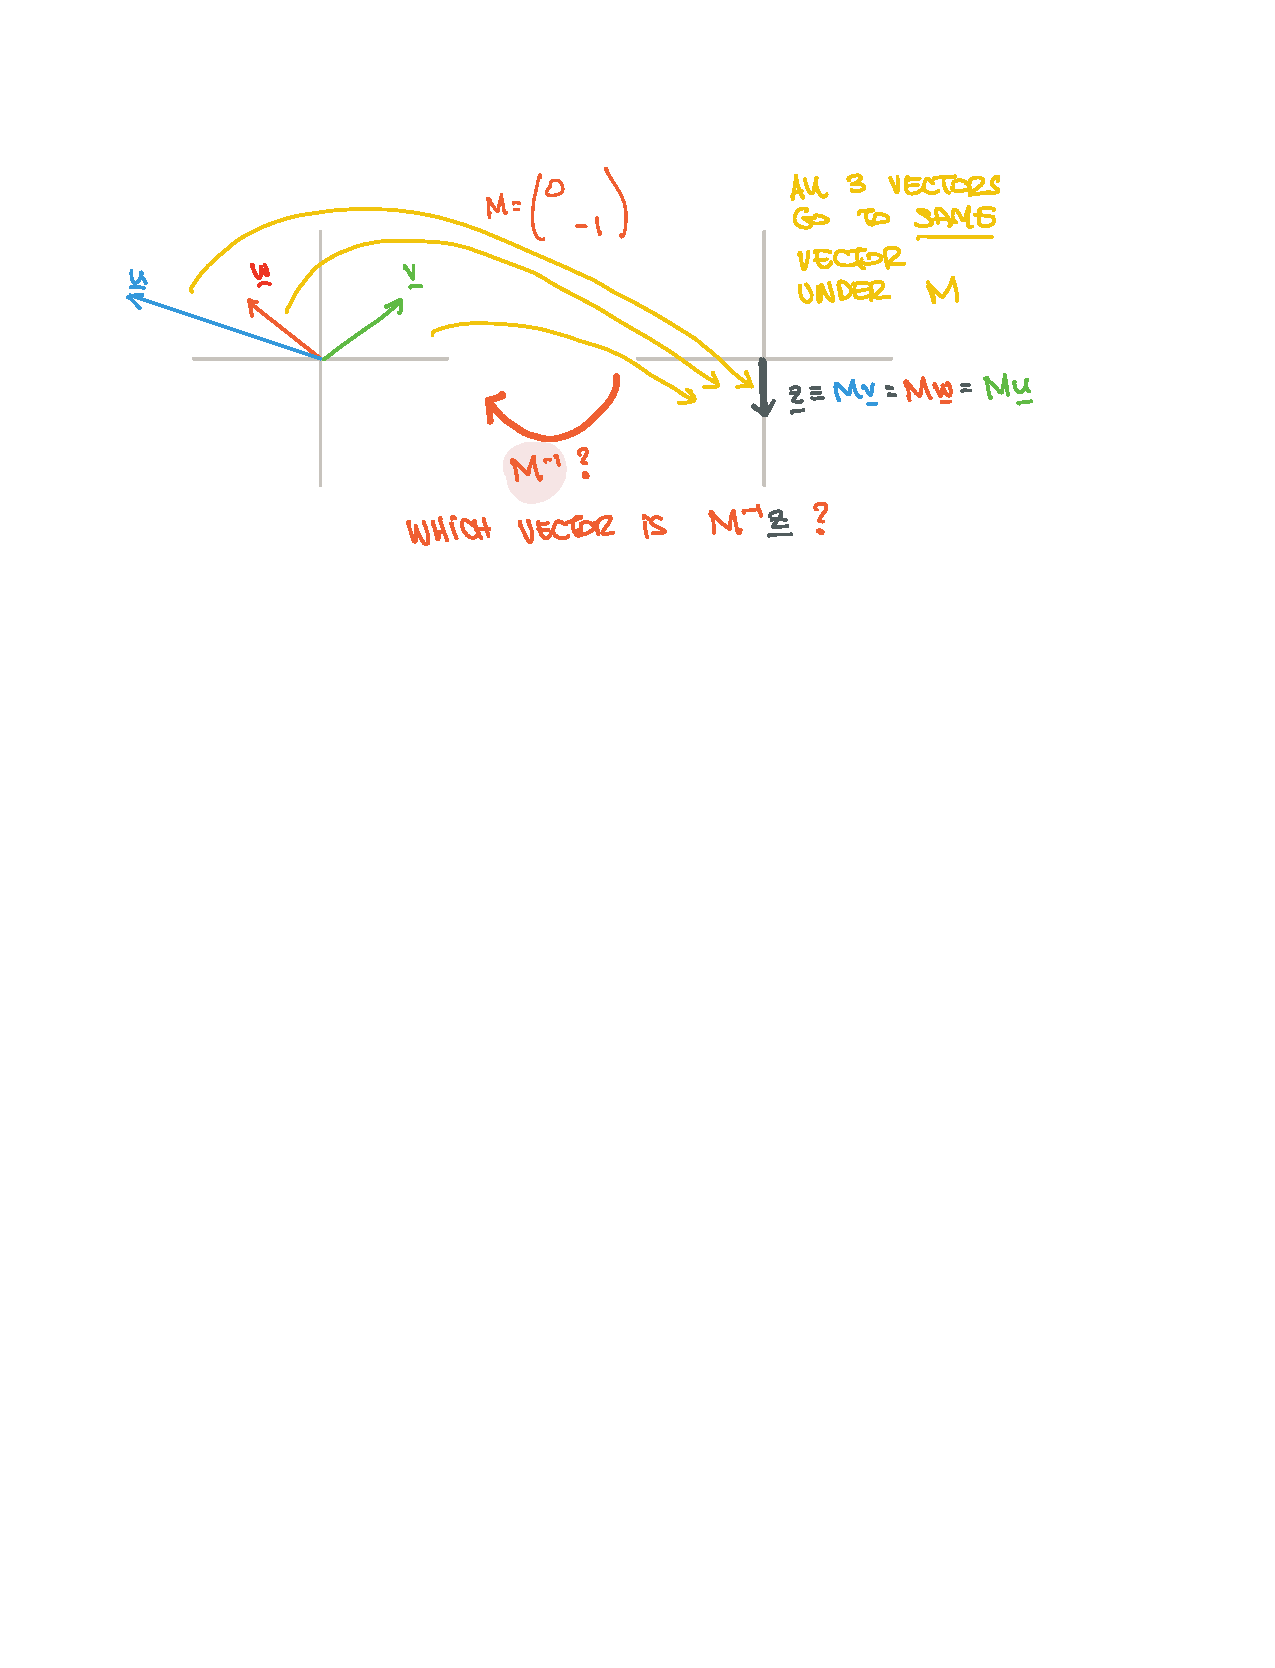
\includegraphics[width=.8\textwidth]{figures/maps_noninv.pdf}
    \caption{$M$ is a non-invertible matrix. We notice that there's no problem applying $M$ to vectors. The odd thing is that there are multiple vectors---$\vec{v}$, $\vec{w}$, and $\vec{u}$ in the picture---that all turn into the same vector, $M\vec{v} = M\vec{w}=M\vec{u}\equiv \vec{z}$. The problem shows up when we try to ``undo'' the transformation $M$ by applying $M\inv$ to $\vec{z}$. $M\inv\vec{z}$ should be a vector. Instead, we have at least three different valid options: $\vec{v}$, $\vec{w}$, and $\vec{u}$. This means that $M\inv$ is not a well defined linear map: it can send one vector $\vec{z}$ into many possible vectors. }
    \label{fig:map:M:no:inv}
\end{figure}
% 
We see the the problem is one of uniqueness. A linear map should take each vector $\vec{v}$ into a single, well-defined vector $M\vec{v}$. $M$ is suspicious because it sends multiple different vectors to the \emph{same} vector, say $M\vec{v} = M\vec{w}$. That's fine. Each of $\vec{v}$ and $\vec{w}$ are sent to \emph{a} vector. The problem shows up when we try to take the inverse. If we write $\vec{z} = M\vec{v} = M\vec{w}$, we know that
\begin{align}
    (M\inv)\vec{z} = (M\inv)M\vec{v} &= \vec{v}
    &
    (M\inv)\vec{z} = (M\inv)M\vec{w} &= \vec{w} \ .
\end{align}
However, we assumed that $\vec{v} \neq \vec{w}$. This means makes the above line inconsistent. The inverse transformation is not defined. Bummer.

Fortunately, most of the \emph{dynamics} in physics \emph{is} invertible. That does not mean that we can ignore non-invertible matrices, though. Non-invertible matrices can be understood as \textbf{projections} onto a subspace. You can see this in the example in Fig.~\ref{fig:map:M:no:inv}. The map $M$ is essentially only using the information about the second component of its input vector and mapping it to just the second component of the output vector. That means that $M$ is really just a map to a one-dimensional subspace. In this way, the two dimensional vector space $\RR ^2$ is \textbf{projected} onto a one-dimensional subspace of $\RR ^2$. In that example, the one dimensional space is defined by vectors of the form
\begin{align}
    \vec{v} = 
    \begin{pmatrix}
    0\\ v^2    
    \end{pmatrix} \ .
\end{align}

Projections are really useful in physics. Sometimes you want to take a big vector space and only focus on a subspace that satisfy certain conditions. For example, it turns out that in nature you can have two types of massless matter particles: left-handed and right-handed according to their quantum spin in the direction of their motion. One may want to project onto only the space of left-handed particles because that is easier to deal with than the entire space. Because projections necessarily ``throw out'' information, they are non-invertible.\sidenote{I think this was more intuitive to past generations of physicists. When you throw out a piece of paper, it ends up in a recycling plant and it gets torn up and is lost forever. Since the advent of computers, when you ``throw out'' a file, you can usually control/command-z and undo to bring it back.}

\begin{example}
One of the most curious puzzles in fundamental physics over the last half century is the black hole information paradox.\footnote{\url{https://www.quantamagazine.org/the-most-famous-paradox-in-physics-nears-its-end-20201029/}} One way of stating the paradox is the question of whether or not ``falling into a black hole'' is a \emph{projection} that throws out information. 
\end{example}

\subsection{Projections in Bra-Ket Notation}
Recall our resolution of the identity \eqref{eq:resolution:of:the:identity}. Each piece in this sum is a projection. For example, consider $\ket{e_2}\!\bra{e^2}$. This is a matrix that acts on a vector $\ket{v}$, pulls out the second component $v^2$, and then returns a vector in the $\ket{e_2}$ direction with length $v^2$. We can see this mathematically:
\begin{align}
    \ket{e_2}\!\bra{e^2} \; v^i\ket{e_i} \;
    &= 
    v^1\ket{e_2}\!\la{e^2}\mid {e_1}\ra + 
    v^2\ket{e_2}\!\la{e^2}\mid {e_2}\ra +
    v^2\ket{e_2}\!\la{e^2}\mid {e_2}\ra + \cdots
    \\ 
    &= v^2 \ket{e_2} \ ,
    \label{eq:projection:e2:e2}
\end{align}
where we used the defining relation $\la e^i \mid e_j \ra = \delta^i_j$\ . This means we can think of our resolution of the identity, $\ket{e_i}\!\bra{e^i}$ as a sum over projections along each axis. One can call each term in the resolution of the identity, say $\ket{e_2}\!\bra{e^2}$ a projector\sidenote{``\emph{Even though I know someday you're gonna shine on your own / I will be your projector},'' from `Protector' by Beyonc\'e Knowles-Carter in the album Cowboy Carter (2024).} onto a given axis.

\subsection{Projecting One Vector Onto Another}

Suppose you have two vectors, $\ket{v}$ and $\ket{w}$ and you want find the projection of $\ket{w}$ onto $\ket{v}$, as shown in Figure~\ref{fig:gram:projection}. 
\begin{figure}[tb]
    \centering
    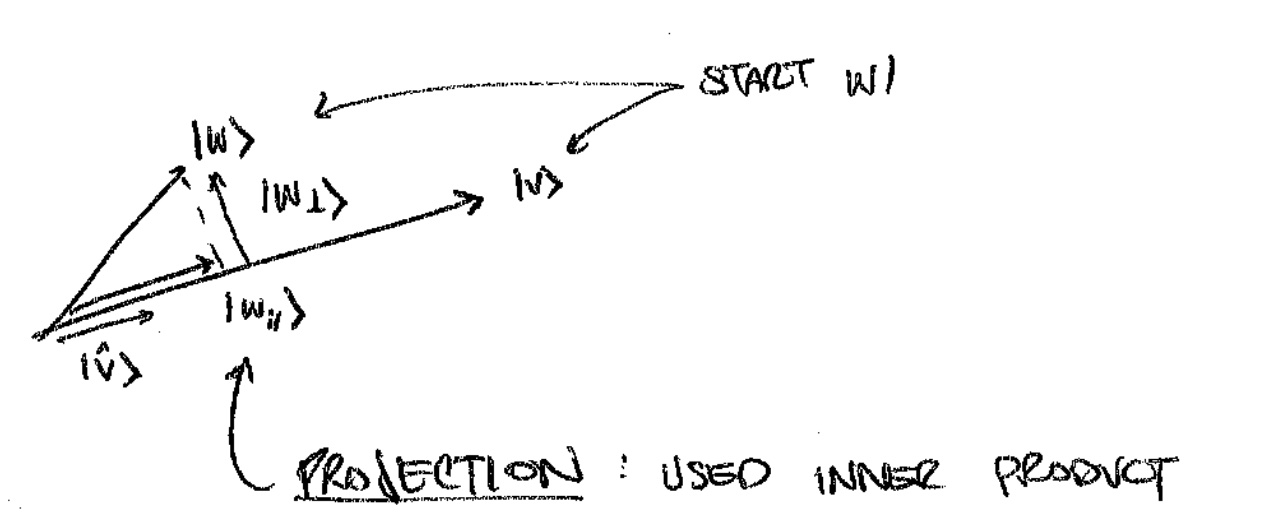
\includegraphics[width=.8\textwidth]{figures/gram-projection.jpg}
    \caption{Projection of a vector $\ket{w}$ onto the axis of another vector, $\ket{v}$.}
    \label{fig:gram:projection}
\end{figure}

Our strategy is to separate the ket $\ket{w}$ into a piece that is parallel to $\ket{v}$ and a piece that is perpendicular to $\ket{v}$,
\begin{align}
    \ket{w}= \ket{w_\paral} + \ket{w_\perp} \ .
\end{align}
The parallel piece $\ket{w_\paral}$ is precisely the projection of $\ket{w}$ onto $\ket{v}$.  The defining characteristic of $\ket{w_\paral}$ is that $\la \hat{w}_\paral, \hat{v}\ra = 1$. That is: the angle between the \emph{unit vectors} is zero---they are parallel. This means that 
\begin{align}
    \ket{w_\paral} \propto \ket{\hat{v}} \ .
\end{align}
What is the proportionality? This is simply the length of $\ket{w}$ along the $\ket{\hat{v}}$ axis, $\la w, \hat v \ra$. Then the statement that $\ket{w_\paral}$ is the vector of length $\la w, \hat v \ra$ in the $\ket{\hat v}$ direction is:
\begin{align}
    \ket{w_\paral} = \la w, \hat{v} \ra \ket{\hat{v}} 
    % =  \ket{\hat{v}}\la \hat{v}, w \ra  
    \ .
\end{align}
We recall from the symmetry of the inner product and our definition of kets \eqref{eq:basis:dual:vectors:as:inner:prod} that we may further write
\begin{align}
    \la w, \hat{v} \ra = \la \hat{v}, w \ra = \la \hat{v} \mid w \ra \ .
\end{align}
What we have done here is written the length of $\ket{w_\paral}$ with respect to a \emph{bra} $\bra{\hat{v}}$ acting on $\ket{w}$. Plugging this back into our expression for $\ket{w_\paral}$, we recover a projection matrix of exactly the form in \eqref{eq:projection:e2:e2}:
\begin{align}
    \ket{w_\paral} = \ket{\hat{v}} \la{\hat{v}} | w \ra  =
    \left(\ket{\hat{v}} \bra{\hat{v}} \right)  \, \ket{w} \ .
     \ .
\end{align}
Evidently $\ket{\hat{v}} \bra{\hat{v}}$ is the matrix that takes $\ket{w}$ and returns $\ket{w_\paral}$, the component of $\ket{w}$ along $\ket{\hat{v}}$. In this language, it is somewhat \emph{obvious} that this is what $\ket{\hat{v}} \bra{\hat{v}}$ does. However, we have not written the components of $\ket{\hat{v}} \bra{\hat{v}}$ in terms of our standard basis. To do that, one simply expands each  of $\ket{\hat{v}}$ and $\bra{\hat{v}}$ in the standard basis. One may invoke linearity to read off the components of the projection matrix, $P = P\aij{i}{j}\ket{e_i}\bra{e^j}$, as seen in the following examples. 



% \begin{example}
% First a simple warm up. Consider the vectors
% \begin{align}
%     \ket{v} &= 2.5 \ket{1}
%     &
%     \ket{w} &= 3\ket{1} + 4\ket{2} \ .
% \end{align}
% We want to find $\ket{w_\paral}$. First we identify the unit vector in the $\ket{v}$ direction, which is simply $\ket{\hat{v}} = \ket{1}$. As a matrix, the projection operator $P = \ket{\hat{v}} \bra{\hat{v}}$ is
% \begin{align}
%     \ket{\hat{v}} \bra{\hat{v}} = \ket{1}\bra{1} 
%     &=
%     \begin{pmatrix}
%         1 & \\
%         & 0
%     \end{pmatrix}
%     \ .
% \end{align}
% Int he last step we have matched the components to  $P = P\aij{i}{j}\ket{i}\bra{j}$.
% Applying this to $\ket{w}$ gives
% \begin{align}
%     \ket{\hat{v}} \bra{\hat{v}}w\ra = \ket{1}\bra{1}\left(3\ket{1}+ 4\ket{2}\right)
%     = 3 \ket{1} \ .
% \end{align}
% \end{example} 


\section{Gram-Schmidt}

The metric allows us to determine whether a basis is orthonormal or not. We \emph{like} orthnormal bases. Sometimes life gives us garbage bases that are not orthonormal. What are we to do? The Gram--Schmidt procedure is a way to use the metric to take any basis and convert it into an orthonormal basis. We already met the key ideas in Section~\ref{sec:projections}. Here we focus on the two dimensional case. Refer back to Fig.~\ref{fig:gram:projection}: we have two vectors, $\ket{v}$ and $\ket{w}$. How do we turn these into two orthonormal basis vectors?
%
The general procedure is:
\begin{enumerate}
    \item Grab one vector from the pile of garbage basis vectors. \emph{Normalize} this vector and stick it in your bag of nice basis vectors. 
    \item Grab another vector from the pile and do whatever you need to do to make it fit as a nice basis vector with the other nice basis vectors in your bag. Start by finding what new `direction' the vector identifies relative to the existing basis vectors. That means finding a direction that is perpendicular\sidenote{It helps to think of this as the part that is not parallel to any existing basis vectors.} to the existing basis vectors. Then normalize the vector pointing in that new direction. The resulting vector can now be placed in the bag of nice basis vectors as an additional orthonormal basis vector.
    \item Repeat the previous step until you have a complete basis. 
\end{enumerate}

We can start with $\ket{v}$ and simply normalize it:
\begin{align}
    \ket{{e}_1}\defeq \ket{\hat{v}}
\end{align}
is the first basis vector. The next step is to take the next vecotr, $\ket{w}$ and pull out the perpendicular part of $\ket{w}$. In Section~\ref{sec:projections} we saw how to do this: simply decompose
\begin{align}
    \ket{w} &= \ket{w_\paral} + \ket{w_\perp}
    &
    \ket{w_\paral} &=  \la {\hat v} , w\ra  \ket{\hat v}  \ .
\end{align}
This gives us $\ket{w_\perp}$ in terms of two vectors $\ket{w}$ and $\ket{w_\paral}$ that we know:
\begin{align}
    \ket{w_\perp} = \ket{w} - \la {\hat v} , w \ra  \ket{\hat{v}} \ .
\end{align}

 We can thus normalize this and that gives us the second basis vector: 
\begin{align}
    \ket{e_2} \defeq \ket{\hat w_\perp}
\end{align}
If you have more vectors, then you can take your next vector and follow the above steps. The only difference with the iterative step is that the decomposition of a vector 
\begin{align}
\ket{u} = \ket{u_\paral} + \ket{u_\perp}    
\end{align}
is such that
\begin{align}
    \ket{u_\paral} = \la \hat{v}, u \ra \ket{\hat{v}} + \la \hat{w}, u \ra \ket{\hat{w}} + \cdots \ ,
\end{align}
where the $\cdots$ represents projections onto all other existing basis vectors. You then normalize the ``leftover'' perpedicular part, $\ket{\hat{u}_\perp}$, and add that to your bag of orthonormal basis vectors.


\begin{exercise}
Would you have the same basis vectors if you started with $\ket{w}$ and then took the perpendicular part of $\ket{v}$? Explain why or why not; your explanation must include a picture illustrating the result.
\end{exercise}


\section{Adjoints}
\label{sec:adjoint}

\begin{quote}
Yes, \emph{this} is the transpose! (c.f.~Figure~\ref{fig:is:this:a:transpose})
\end{quote}

In Section~\ref{sec:transpose} we introduced the \emph{transpose} of a matrix. We noted that while the working definition there is easy to explain, it does not properly capture the core mathematical idea. The reason for this was that we needed to appreciate that matrices are not arrays of numbers, but are linear transformations from vectors into other vectors. The definition that captures this is called the adjoint of a matrix. The \textbf{adjoint}\index{adjoint} of a matrix\sidenote{Here we mean a linear transformations that take vectors to vectors.} $M$ is written $M^\dag$ and is defined by the relation
\begin{align}
    \la M^\dag w, v \ra = \la w, M v \ra \ . 
\end{align}
Using the pre-filled inner product definition of dual vectors \eqref{eq:dual:vec:is:pre:filled:inner:product}, we may rewrite this as
\begin{align}
    \la M^\dag w \mid v \ra = \la w \mid M v \ra \ .
\end{align}
We show below that for real vector spaces, $M^\dag$ is precisely the transpose $M^\trans$. However, this definition generalizes to complex vector spaces where $M^\dag$ is called the \textbf{Hermitian conjugate}. We use the $M^\dagger$ notation to emphasize the utility of this more general definition. 

\begin{marginfigure}%[th]
    
\includegraphics[width=\textwidth]{figures/MordorIndices.jpg}
    \captionsetup{font={scriptsize,sf}}
    \caption{``One does not simply walk into Mordor'' meme, adapted to the transpose. Generated at \url{https://imgflip.com/i/8opffm}.}
    \label{fig:transpose:mordor}
\end{marginfigure}
\begin{example}[One does not simply swap the indices] See Figure~\ref{fig:transpose:mordor}. What could possibly go wrong with the usual ``swap the indices'' definition of the transpose? The problem is that in our sophisticated upper/lower index notation, we need to deal with the height of the indices. Matrices have their first index upper and their second index lower. If $M=M\aij{i}{j}\ket{i}\bra{j}$, then what is the appropriate index structure of the transpose?
\begin{align}
    M^\trans \stackrel{?}{=} 
    \begin{cases}
    (M^\trans)\aij{j}{i}\ket{j}\bra{i}    & \text{ or }\\
    (M^\trans)_{j}^{\phantom{j}i}\ket{i}\bra{j}
    \end{cases}
    \quad\text{.}
\end{align}
The adjoint gives us a way to make sense of this rigorously. The existence of a metric is critical in this analysis. 
\end{example}

\begin{example}
By the symmetry of the metric we could have equivalently written
\begin{align}
    \la M^\dag \vec{w}, \vec{v} \ra =
    \la \vec{w} ,  M \vec{v} \ra =
    \la \vec{v}, M^\dag \vec{w} \ra =
    \la M \vec{v}, \vec{w} \ra 
    \ .
\end{align}


The point of the metric is \emph{not} that you're moving the matrix $M$ from one slot to the other, it is that you are changing from a transformation $M$ that acts on $\ket{v}$ to a transformation $M^\dag$ that acts on the \emph{other} input vector $\ket{w}$ defined such that the inner product is the same.
\end{example}

\subsection{The indices of the `transpose'}
When $M$ is a real matrix, we usually say $M^\dag \equiv A^\trans$. What does this \emph{mean}? Write out the components of each side:
\begin{align}
    \la M^\dag v, w \ra
    &=
   w^k \, g_{ki}  (M^\dag)\aij{i}{\ell} v^\ell  \,  
    &
    \la  v,M w \ra
    &=
   v^\ell\, g_{\ell j}  M\aij{j}{k} w^k  
   \ .
   \label{eq:adjoint:transpose:int1}
\end{align}
Now set these two inner products equal to each other gives\sidenote{Here we have canceled $w^kv^\ell$ on both sides. The result is correct, but this justification is suspect because the $k$ and $\ell$ indices are summed over. What we have really done is used the fact \eqref{eq:adjoint:transpose:int1} is true for \emph{all} allowed $w^k$ and $v^\ell$ so that the rest of the equality cannot depend on those factors. Indeed, the equality \eqref{eq:adjoint:transpose:int1} must be true for \emph{each} $k$ and $\ell$. This is a subtle argument that lets use do a slick manipulation. It is worth thinking carefully about it.}
\begin{align}
    g_{ki}(M^\dag)\aij{i}{\ell}
    &=
    g_{\ell j} M\aij{j}{k}
    \label{eq:adjoint:transpose:int2}
\end{align}
Contracting both sides with the inverse metric $g^{km}$ gives
\begin{align}
    (M^\dag)\aij{m}{\ell} &= g_{\ell j} M\aij{j}{k} g^{km} \ .
    \label{eq:adjoint:def}
\end{align}
This relation \emph{defines} the components adjoint, $(M^\dag)\aij{i}{j}$. We see that the adjoint has the normal index structure of a linear transformation: first index raised, second index lowered. Further, when the metric is diagonal, it is clear that the first index of $M^\dag$ corresponds to the second index of $M$ and vice  versa. In this sense, the order of the indices have swapped.  In fact, the right-hand side of  \eqref{eq:adjoint:def} can be written with the metric implicit:
\begin{align}
    g_{\ell j} M\aij{j}{k} g^{km} \equiv 
    M_\ell^{\phantom{\ell}m} \ ,
\end{align}
though we shall avoid this notation since it is a bit uncommon.



\begin{exercise}
In your own words, articulate the difference between a matrix $A$, its inverse $A\inv$, and its transpose $A^\trans$. What if $A$ is a rotation?
\end{exercise}

\begin{exercise}
Show that taking the adjoint twice returns you to the original matrix, $(A^\dag)^\dag = A$.
\end{exercise}

% \begin{example}
% The adjoint also gives us another way to understand why isometries act differently on column vectors (ket) versus row vectors (bra). The metric lets us convert a column vectors into row vectors, as we saw in Section~\ref{sec:machine:to:make:row:vectors}. Start with a vector $\ket{v}$ with components $v^i$. Under a rotation, these components become $(v')^i = R\aij{i}{j}v^j$. From the transformed ket $\ket{v'} = (v')^i \ket{e_i}$ we invoke the metric to convert this into a bra:
% \begin{align}
% \bra{v'} = \la v', \smallslot \ra = \la \smallslot, v' \ra \equiv v'_i \bra{i} \ .    
% \end{align}
% In the last line we have implicitly used the metric: we have a definition for $(v')^i$, so the meaning of $(v')_i$
% is understood to be
% \begin{align}
%     (v')_i = g_{ij} R\aij{j}{k}v^k \ .
% \end{align}
% What are the components of $(v')_i$ relative to $v_i$? To do that we can insert $\one$ in a clever way:
% \begin{align}
%     g^{mn}g_{n\ell} = \delta^m_\ell
% \end{align}
% so that 
% \begin{align}
%     (v')_i = g_{ij} R\aij{j}{k} g^{k\ell}g_{\ell m} v^m
%     = 
%     \left(g_{ij} R\aij{j}{k} g^{k\ell}\right)
%     v_\ell
%     = 
%     v_\ell(R^\dag)\aij{\ell}{i} 
%     \ ,
% \end{align}
% where again we have implicitly \emph{defined} $v_\ell = g_{\ell m}v^m$. That's just what metrics do. That's what they \emph{do}.\footnote{\url{https://www.youtube.com/watch?v=Akq0xeu-RHE}} In the last equality we recognize the definition of the adjoint, \eqref{eq:adjoint:def}. In our case of a real metric space, of course, this is simply $R^\dag = R^T$. This confirms for us that the objects with lower indices transform by contracting with $R^\dag$, which we identified in \eqref{eq:rotation:definition:one} to be the inverse of the rotation $R$. So there you have it: objects with lower indices transform with $R\inv = R^\dag$. 

% We can do a sanity check for this. The inner product is a number and should not transform under rotations. We can see what happens:
% \begin{align}
%     \la v , w \ra \to \la Rv, Rw \ra = \la v, R^\dag R w \ra = \la v, w \ra \ .
% \end{align}
% where we used $R^\dag R = \one$. 




% % Starting with a ket $\ket{v}$, we define the bra
% % \begin{align}
% % \bra{v} = \la v, \smallslot \ra = \la \smallslot, v \ra \ .    
% % \end{align}
% % Now act $\bra{v}$ on a ket $\ket{w}$. By linearity, I can also transform the ket by a matrix $A$ and then feed $\ket{Aw}=A\ket{w}$ to $\bra{v}$:
% % \begin{align}
% %     \la{v} | {Aw} \ra = \bra{v}A \ket{w} = \la v, Aw \ra \equiv \la A^\dag v, w\ra = \bra{A^\dag v} w\ra \ .
% % \end{align}
% % Now suppose $A$ is an isometry. Assuming that the space is real\footnote{That is: every time we say `number' we mean a \emph{real} number, $\RR$.} and that we have the Euclidean metric, this is simply the assumption that $A=R$, a rotation. 
% \end{example}

\subsection{Self-Adjoint}

There is a special class of matrices that are called \textbf{self-adjoint}\index{self-adjoint} or, equivalently, \textbf{Hermitian}\index{Hermitian}. For real matrices, this turns out to simply mean that they are \emph{symmetric}. These are matrices $M$ for which 
\begin{align}
    M^\dag = M \ .
\end{align}
We shall come to appreciate that these matrices not only have nice properties, but that they are precisely the types of matrices that play significant roles in physics.

We can see that self-adjoint matrices are symmetric. The definition of self-adjoint is:
\begin{align}
    \la M w, v \ra = \la w, M^\dag v \ra = \la w, M v \ra \ .
\end{align}
By the symmetry of the metric, we also have 
\begin{align}
    \la M w, v \ra = \la v, Mw \ra \ .
\end{align}
Combining these gives, for a self-adjoint matrix $M$,
\begin{align}
    \la w, M v \ra = \la v, Mw \ra \ .
\end{align}
We apply this result to basis vectors, $\ket{w} = \ket{e_i}$ and $\ket{v} = \ket{e_j}$ for some $i$ and $j$. Recall the \emph{pre-loaded inner product} definition of basis dual vectors in \eqref{eq:basis:dual:vectors:as:inner:prod}: $\bra{e^i} = \la e_i, \slot \ra$, we may write our self-adjoint definition as\sidenote{To be clear: the arguments of the inner product are vectors. This means that $Me_i$ as one of the arguments means $M\ket{e_i}$. } 
\begin{align}
    \la e_i,  Me_j \ra &= \la e_j, M e_i \ra \\
    \la e_i \mid M \mid e_j \ra &= \la e_j \mid M \mid e_i\ra\\
    M\aij{i}{j} &= M\aij{j}{i}
    \ .
    \label{eq:self:adjoint:is:symmetric}
\end{align}
Do not be confused by the notation: 
\begin{enumerate}
    \item $\la e_i \mid M \mid e_j \ra$ simply means that $M$ acts on the vector $\ket{e_j}$ to produce a vector $\ket{Me_j}$. Then the dual vector $\bra{e_j}$ acts on $\ket{Me_j}$ to produce a number.
    \item The number that is produced from $\la e_i \mid M \mid e_j \ra$ is the $j$--$i$ component of $M$. You can see this because the components of $\ket{e_i}$ are zero everywhere and one on the $i^\textnormal{th}$ component. (See example below.)
\end{enumerate}

\begin{example}
In matrix multiplication notation, we may write:
\begin{align}
    \begin{pmatrix}
        0 & 1
    \end{pmatrix}
    \begin{pmatrix}
        M\aij{1}{1} & M\aij{1}{2}\\
        M\aij{2}{1} & M\aij{2}{2}
    \end{pmatrix}
    \begin{pmatrix}
        1 \\ 0
    \end{pmatrix}
    &= 
    M\aij{2}{1} \ .
\end{align}
\end{example}

You may feel justifiably uncomfortable that in \eqref{eq:self:adjoint:is:symmetric} we ended up with an equation where the heights of the $i$ and $j$ indices on the left-hand side do not match with those on the right-hand side. This happened because the \emph{pre-loaded inner product} effectively raises the index of a basis vector. It is a bit of a notational quandry and has to do with the metric's role as an index lower-er or raise-er. If you wish to be more comfortable with this, you can treat \eqref{eq:self:adjoint:is:symmetric} as a component-wise identity. Alternatively, you may think about it component-wise using \eqref{eq:adjoint:def}: a self-adjoint operator has $(M^\dag)\aij{i}{j} = M\aij{i}{j}$. There are factors of the metric that account for raising and lowering the indices.


\begin{subappendices}

\section{A Matrix in Another Basis}

Consider a linear transformation from vectors to vectors, $A$. In a given basis, this linear transformation is represented as a matrix.\sidenote{I sometimes write `linear transformation' and `matrix' interchangeably. Formally the matrix is the array of numbers that is indicated by indices, whereas the linear transformation is the index-less operation that does not assume a basis.} Often one would like to describe the components of the matrix in a different basis. Here's how one converts from the components $A\aij{i}{j}$ in the $\ket{e_{i}}$ basis to its components $\tilde A\aij{a}{b}$ in a different basis, $\ket{f_a}$.\sidenote{Please review Section~\ref{sec:basis:of:matrices} to recall why the ket-bra is the natural basis of matrices.}
\begin{align}
    A &= A\aij{i}{j}\ket{e_i}\!\bra{e^j}
    \\&=
    A\aij{i}{j}\quad
    \one
    \ket{e_i}\!\bra{e^j}
    \one
    \\&=
    A\aij{i}{j}\quad
    \ket{f_a}\!\la {f^a} \mid 
     {e_i} \ra\!  \la {e^j} \mid
    {f_b}\ra \!\bra{f^b}
    \\&=
    \la {f^a} \mid 
     {e_i} \ra
    A\aij{i}{j}
    \la {e^j} \mid
    {f_b}\ra
    \quad
    \ket{f_a}\!\bra{f^b}
\end{align}
Now please review Figures~\ref{fig:basis:change:ef} and \ref{fig:basis:change:fe}. We realize that the numbers $\la {f^a} \mid 
     {e_i} \ra$ and $\la {e^j} \mid
    {f_b}\ra$ are simply components of the rotation matrix between the two bases. Picking a convention\sidenote{You could have swapped which one is $R$ and which is $R\inv$. After all, the inverse of a rotation is simply a rotation in the opposite direction.} for which one we call $R$ and which we call $R\inv$ gives:
\begin{align}
    A &= (R\inv)\aij{a}{i}
    A\aij{i}{j}
    R\aij{j}{b}
    \quad
    \ket{f_a}\!\bra{f^b} 
    \\&\equiv
    \tilde A\aij{a}{b}
    \quad
    \ket{f_a}\!\bra{f^b}
    \ .
\end{align}
This means that the matrix components $\hat A\aij{a}{b}$ in the $\ket{f_{1,2}}$ basis are related to the matrix components $A\aij{i}{j}$ in the $\ket{e_{1,2}}$ basis by
\begin{align}
    \tilde A\aij{a}{b} &= (R\inv)\aij{a}{i}
    A\aij{i}{j}
    R\aij{j}{b}
    &
    A\aij{i}{j} = R\aij{i}{a}\tilde A\aij{a}{b}(R\inv)\aij{b}{j} \ .
\end{align}



\section{Discrete isometries}
\label{sec:discrete:isometries}

One of the notable features of rotations is that you can rotate by any continuous amount, $\theta$. You can rotate by $\theta=\pi/2$, or $\theta = \pi/2 + \varepsilon$ for, say, $\varepsilon = .0001$. Thus the rotation matrix parameterizes an infinite number of possible rotations. Because there is a continuous parameter for the amount by which one performs a rotation, we say that this is a continuous isometry. There are, however, often \emph{discrete} isometries where there is simply a handful of matrices under which the metric is invariant. In Euclidean two dimensional space, one such matrix is 
\begin{align}
    P = \begin{pmatrix}
        1 & \\
        & -1 
    \end{pmatrix} \ .
\end{align}
Under $P$, the second component of a vector (in the standard basis) changes sign. Because the metric transforms with two factors of $P$---here we use $P^\dag = P$---it remains unchanged:
\begin{align}
    P^\text{T}gP = 
    \begin{pmatrix}
        1 & \\ 
        & -1 
    \end{pmatrix}
    \begin{pmatrix}
        1 & \\ 
        & 1 
    \end{pmatrix}
    \begin{pmatrix}
        1 & \\ 
        & -1 
    \end{pmatrix}
    = 
    \begin{pmatrix}
        1 & \\ 
        & 1 
    \end{pmatrix} \ .
\end{align}
\begin{exercise}
Suppose that the components of the metric in $\RR^2$ are not diagonal. That is, $g_{12} = g_{21}\neq 0$. Is $P$ an isometry of this metric space?
\end{exercise}

The total set of isometries is every combination of rotations and discrete transformations. We often say that this is a \textbf{group}\index{group}. One may write a generic isometry as a product of rotations and discrete transformations. 
\begin{example}
The following transformation is a combination of a discrete transformation $P$ and a rotation:
\begin{align}
    \tilde R = PR =
    \begin{pmatrix}
        1 & \\ 
        & 1 
    \end{pmatrix}
    \begin{pmatrix}
        c & -s\\ 
        s & \pp c
    \end{pmatrix}
    =
    \begin{pmatrix}
        c & -s\\ 
        -s & - c
    \end{pmatrix} \ .
    \label{eq:discrete:isometry:eg}
\end{align}
This matrix does \emph{not} look like a rotation. The diagonal elements differ by a sign, while the off-diagonal elements are the same. If we did not know about discrete isometries, we would have said that this matrix does not map one orthonormal basis to another. In fact, it does.
\end{example}
\begin{exercise}
Compare the rotation-and-discrete transformation in \eqref{eq:discrete:isometry:eg} to a transformation that is simply a rotation. For concreteness, pick a rotation angle $\theta = \pi/4$ so that $c=s=1/\sqrt{2}$. Apply the rotations $R$ and $\tilde R$ to the standard basis. How do the ``rotated'' bases differ?
\end{exercise}

In three dimensions this notion shows up as \emph{parity}. Here are two ways to represent the parity transformation in three dimensions:
\begin{align}
    P &=
    \begin{pmatrix}
        -1 & & \\
        & -1 & \\
        & & -1
    \end{pmatrix} 
    &
    P =
    \begin{pmatrix}
        1 & & \\
        & 1 & \\
        & & -1
    \end{pmatrix}
    \ .
\end{align}
The reason why there are different ways to represent this discrete symmetry is that the two are related by a rotation. 
\begin{exercise}
Describe---in words or drawing if that is simpler---the rotation that relates the two parity matrices above. It may help to think about what each representation of $P$ does to the standard basis vectors. 
\end{exercise}

You can tell that the two are related by a rotation if you think about all that ``right hand rule'' stuff you learned when you first did angular momentum in mechanics. The right hand rule enforced a certain \emph{orientation} of your basis vectors. The positive $x$, $y$, and $z$ directions are chosen to have a particular orientation: if you curl the fingers of your right hand from the $x$-axis to the $y$-axis, then your thumb is pointing in the $z$ direction. You can rotate your hand in any way, but this orientation stays the same. Similarly, if you are contrarian and decided to define your axes by a ``left hand rule,'' then (1) several of your angular momentum-related results are off by a minus sign, and (2) there is no way to rotate your left hand to make it match the orientation of your right hand. This notion is pervasive in nature in three spatial dimensions: fundamental particles have a spin that defines an orientation that is either left- or right-handed. Even protein can have a \emph{chirality} where identical sequences of amino acids may spiral in one direction or another---and biological life on earth can only use one orientation and not the other. 

By manipulating objects (like your right hand) you have an intuitive sense of rotations in three-dimensions. What may be less obvious is that you also have a simple tool for understanding what a parity transformation does: look in the mirror. If you raise your right hand, then the image of you in the mirror raises their left hand. If you do physics with a right-handed coordinate system, then your mirror image will do physics in a left-handed coordinate system. You can bet that the image of you is composed of proteins with the opposite chirality and subatomic particles spinning in the opposite orientation. 
\begin{exercise}
Explain why your image in a mirror exchanges left and right but does not swap up and down.\footnote{This is a question that was posed in my freshman physics class. It was not the first time that I heard the question, but I was surprised that it is a mathematical question in the realm of physics. I have since come to appreciate the significant role that parity plays in many aspects of physics. I hope that soon you will as well.}
\end{exercise}



\end{subappendices}
